Sistem navigasi ini dirancang untuk beroperasi pada area yang petanya sudah diketahui
sebelumnya (\emph{known map}). Informasi lingkungan tersebut disimpan dalam bentuk
\emph{occupancy grid}.
Tantangan utama yang dihadapi adalah bahwa data lingkungan yang dikumpulkan
bersifat tiga dimensi (3D), sementara \emph{occupancy grid} yang digunakan hanya
memiliki dua dimensi (2D). Untuk menyetarakan perbedaan ini, lingkungan 3D
dibagi menjadi beberapa \emph{region} yang lebih kecil, dan setiap \emph{region}
direpresentasikan secara terpisah dalam bentuk peta 2D. Sehingga, setiap
\emph{region} menjadi proyeksi 2D dari sub-bagian lingkungan 3D. Pembagian \emph{region}
dalam ruang 3D dapat dilihat pada Gambar~\ref{fig:sim_world}.

Selain peta utama, sistem navigasi juga membutuhkan peta transisi yang berfungsi
sebagai jembatan penghubung antar \emph{region}. Peta transisi adalah peta terpisah
yang menyimpan informasi relasi spasial setiap \emph{region} terhadap \emph{global
frame of reference} yang seragam, sehingga posisi absolut masing-masing \emph{region}
dalam koordinat global dapat diketahui. Dengan adanya peta transisi ini, robot dapat
melakukan perpindahan antar \emph{region} secara mulus selama navigasi, meskipun
kedua \emph{region} terpisah oleh area \emph{unknown}. 

\begin{figure}[H]
\centering
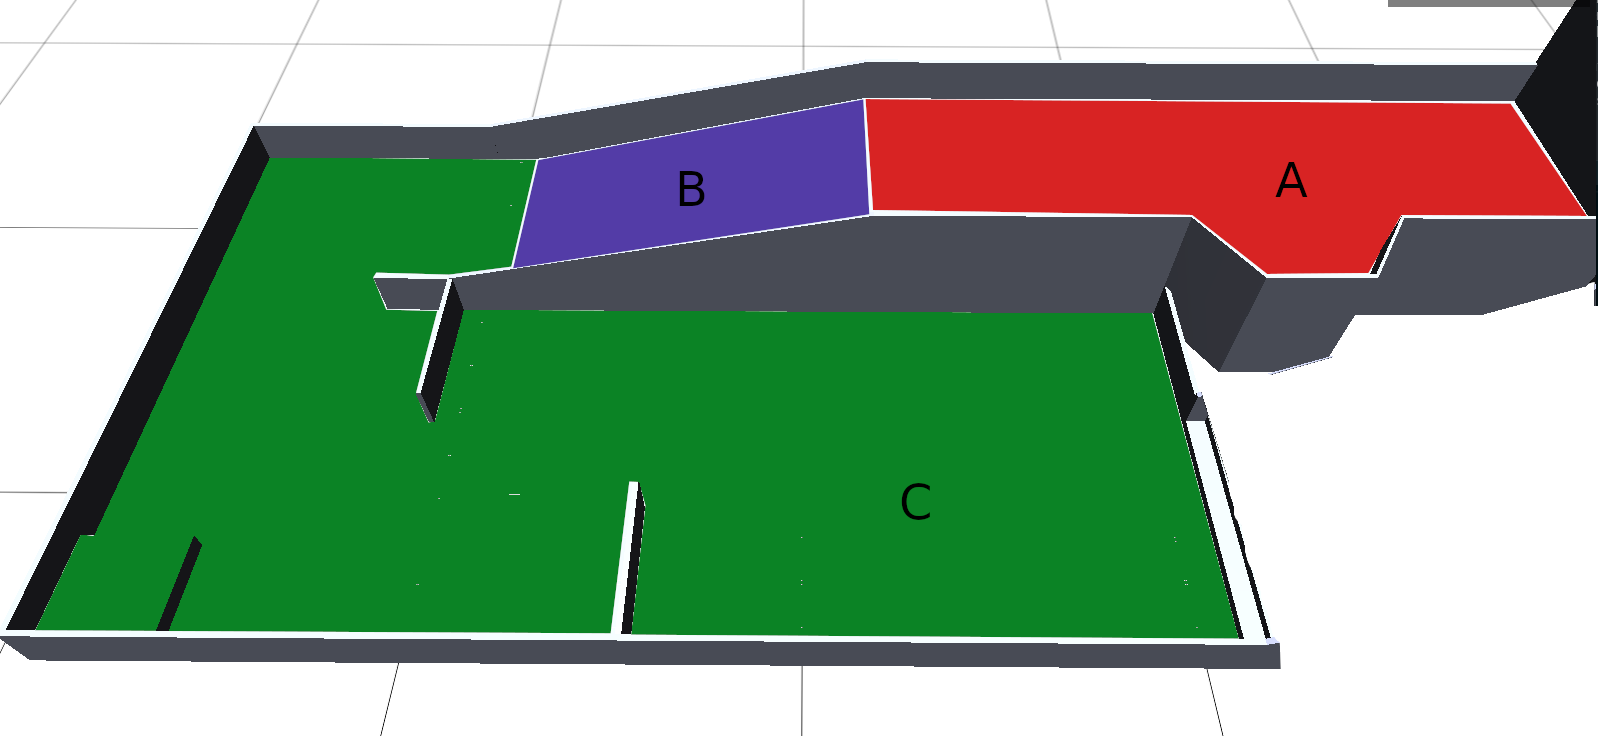
\includegraphics[width=0.7\textwidth]{gambar/sim_world.png}
\caption{Lingkungan arena dalam 3D}
\label{fig:sim_world}
\end{figure}

\subsection{Map Region}

Peta untuk setiap \emph{region} diperoleh melalui proses \emph{mapping}  menggunakan Hector SLAM atau dibuat secara manual berdasarkan dimensi ukuran lingkungan asli. Hasil akhir peta masing-masing \emph{region} ditunjukkan pada Gambar \ref{fig:tiga_gambar}.

\begin{figure}[H]
\centering
\begin{subfigure}{0.3\textwidth}
    \centering
    
\includegraphics[trim={1cm 1cm 1cm 1cm}, clip, width=\textwidth]{gambar/map_R1_edit.png}
    \caption{Map Region A}
    \label{fig:gambar1}
\end{subfigure}
\hfill
\begin{subfigure}{0.3\textwidth}
    \centering
    
\includegraphics[width=\textwidth]{gambar/map_R2_real.png}
    \caption{Map Region B}
    \label{fig:gambar2}
\end{subfigure}
\hfill
\begin{subfigure}{0.3\textwidth}
    \centering
    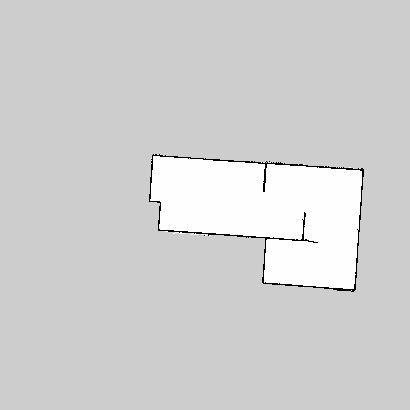
\includegraphics[width=\textwidth]{gambar/map_r10_edit.png}
    \caption{Map Region C}
    \label{fig:gambar3}
\end{subfigure}
\caption{Map Occupancy Grid masing-masing region}
\label{fig:tiga_gambar}
\end{figure}

Sistem navigasi tidak menggunakan peta individu dari masing-masing \emph{region} secara terpisah, melainkan menggunakan satu peta utama yang merupakan hasil kombinasi seluruh \emph{region}. Dalam peta utama tersebut, setiap \emph{region} dipisahkan oleh area \emph{unknown} (wilayah yang tidak diketahui).

\begin{figure}[H]
\centering
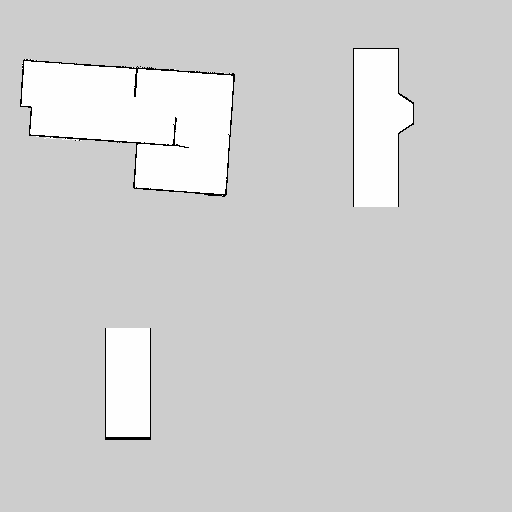
\includegraphics[width=0.4\textwidth]{gambar/combined_map.png}
\caption{Map Gabungan}
\label{fig:combined_map}
\end{figure}

Untuk menghasilkan map gabungan, diperlukan deteksi Region of Interest (ROI) pada setiap peta pisah.
ROI didefinisikan sebagai area yang mengandung piksel gelap (nilai < threshold), yang mewakili obstacle atau peta yang bermakna. Untuk setiap peta, ROI diidentifikasi melalui:

$$\text{ROI} = \{(x,y) : I(x,y) < T\}$$

dimana, $I(x,y)$ adalah nilai intensitas piksel pada koordinat $(x,y)$,
$T$ adalah threshold

Peta gabungan akhir tersusun dari beberapa bagian, dan setiap bagian ditempati
oleh satu \emph{region}. Banyaknya bagian tersebut ditentukan oleh jumlah peta
\emph{region} yang dimasukkan ke dalam proses penggabungan.

\subsection{Map Transisi}

\begin{figure}[H]
\centering
\begin{subfigure}{0.3\textwidth}
    \centering
    
\includegraphics[width=\textwidth]{gambar/transition_map.png}
    \caption{Map transisi}
    \label{fig:transition_map}
\end{subfigure}
\qquad
\begin{subfigure}{0.3\textwidth}
    \centering
    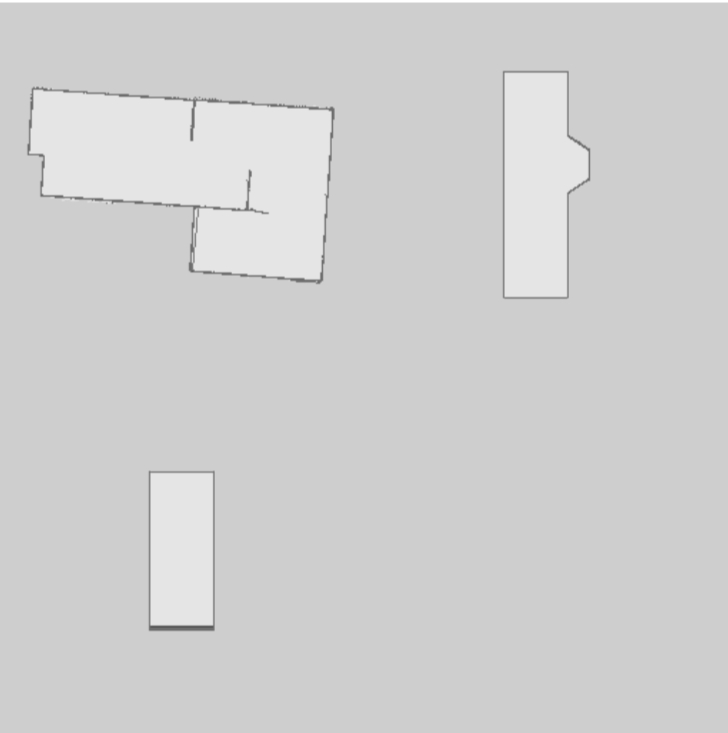
\includegraphics[width=\textwidth]{gambar/transition_map_overlay.png}
    \caption{Map transisi dengan overlay region}
    \label{fig:transition_map_overlay}
\end{subfigure}
\caption{Map transisi antar region}
\label{fig:transition_map_all}
\end{figure}

Peta transisi digunakan untuk menandakan perbedaan antara

 

% ```
% 1. Buka program dengan map YAML
%    ↓
% 2. Tekan '1' → Mode Select Region A
%    ├─ Klik untuk menambah piksel Region A
%    ├─ Garis preview tampil antara click terakhir dan mouse
%    └─ Tekan '1' lagi → Selesai Region A
%    ↓
% 3. Tekan '2' → Mode Select Region B
%    ├─ Klik untuk menambah piksel Region B
%    ├─ Garis preview tampil antara click terakhir dan mouse
%    └─ Tekan '2' lagi → Selesai Region B
%    ↓
% 4. Sistem otomatis membuat pair Region A-B
%    ↓
% 5. Ulangi langkah 2-4 untuk wormhole connection lainnya
%    ↓
% 6. Tekan 's' → Simpan semua data
%    ├─ Buat transition_map.pgm
%    └─ Buat transition_map.yaml
%    ↓
% 7. Program selesai